\subsubsection{Details Analysis of One Instance from Generator}
~\par
Based on the generator, we have tested lots of data and compare the performance of different algorithm. Data is random and different from time to time and we cannot show all of them in the paper, but most of them can reveal the similar performance of these algorithms, so we select one of the most representative data and analyse different performance of algorithms.To better analyse the performance, we introduce a random algorithm and regard the result of it as the baseline.
\begin{enumerate}
    \item Performances:~\par~\par
    % Table generated by Excel2LaTeX from sheet 'Sheet1'
\begin{tabular}{|c|c|c|c|}
\hline
\multicolumn{4}{|c|}{Basic Mathematics Characteristics of Performance} \bigstrut\\
\hline
Methods & Average Time & Maximal Finish Time & Standard Deviation \bigstrut\\
\hline
Random Approach & 30.823 & 107.331 & 22.6757 \bigstrut\\
\hline
Greedy Approach & 24.203 & 106.76 & 20.8664 \bigstrut\\
\hline
K-Greedy Approach & 24.8509 & 114.503 & 22.8843 \bigstrut\\
\hline
Network-Flow-Based Greedy Approach & 23.4635 & 90.35 & 19.2471 \bigstrut\\
\hline
Network-Flow-Based Fair Approach & 23.6664 & 81.33 & 18.4392 \bigstrut\\
\hline
\end{tabular}%

    ~\par~\par~\par
    \item Figures of the data. (Fig.\ref{fig-hist}, Fig.\ref{fig-residual})
    ~\par
    \begin{figure}[htb]
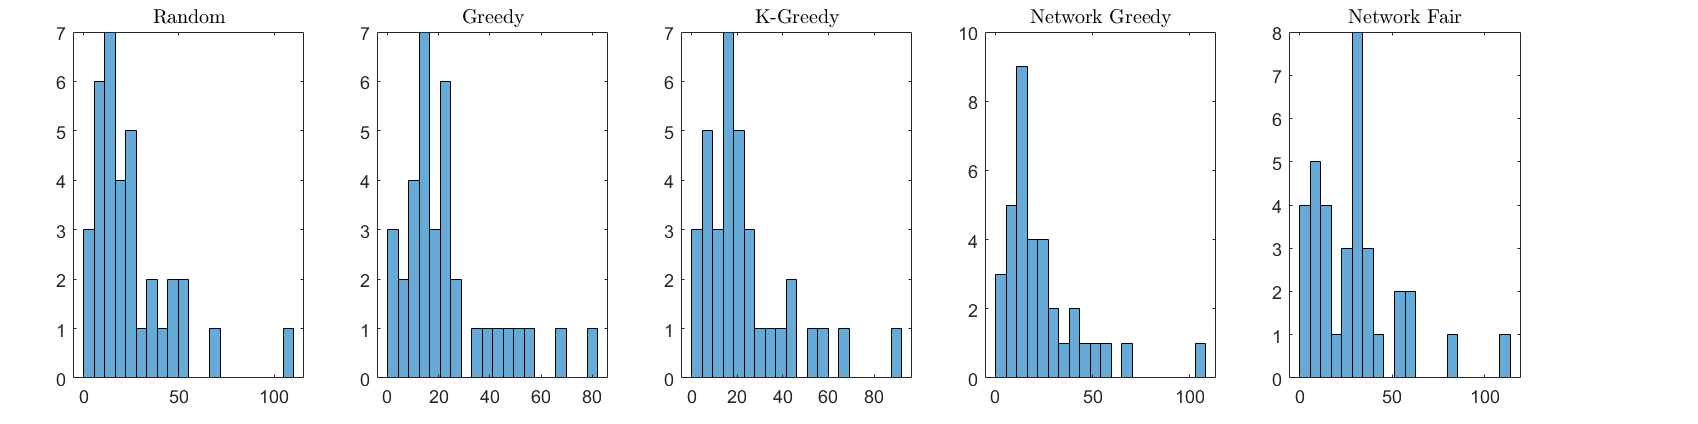
\includegraphics[width=1.1\textwidth]{figure/fig-hist.png}
\centering
\caption{Histogram of Jobs Finish Time in Different Algorithms} \label{fig-hist}
\end{figure}
    \begin{figure}[htb]
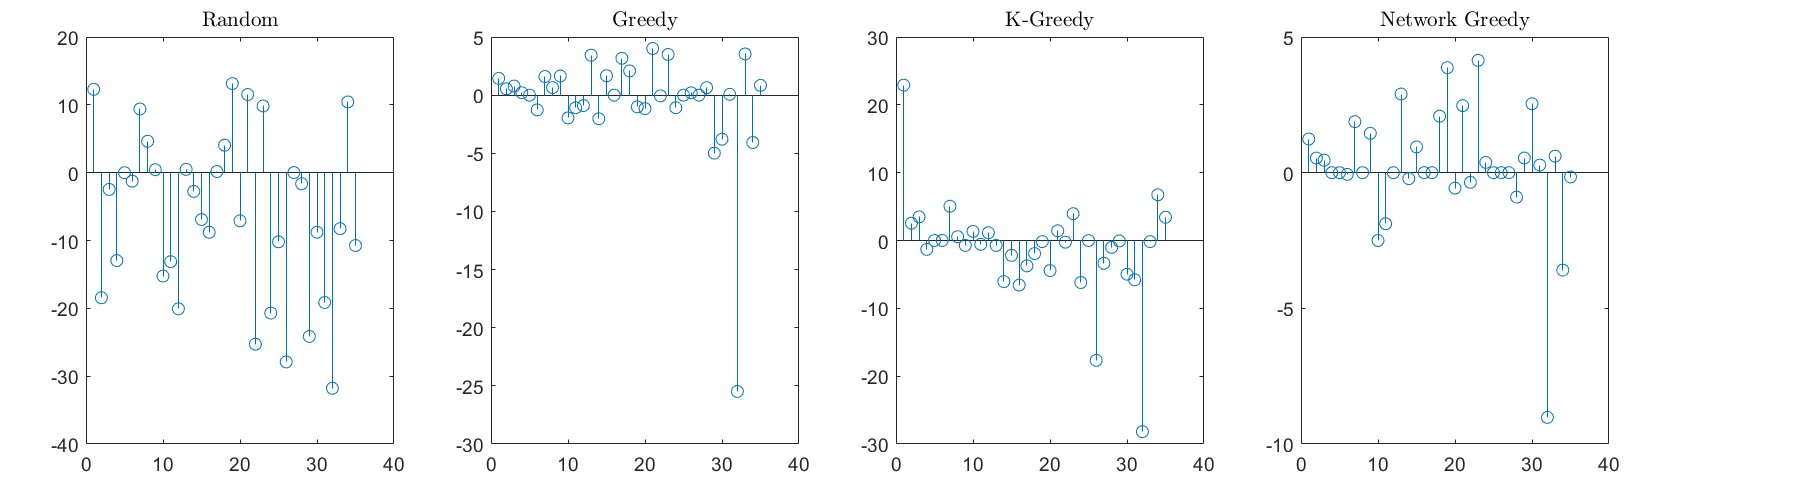
\includegraphics[width=1.1\textwidth]{figure/fig-residual.png}
\centering
\caption{Residual of Jobs Finish Time. Network-Flow-Based Fair Approach vs Others.} \label{fig-residual}
\end{figure}
    \item Results analysis:
    \begin{enumerate}
        \item Average time of the jobs:\\
        Comparing to the baseline, all of the algorithms have optimized the running time of each jobs and tasks. However, for most of time, the average time of different algorithms have no distinct different. That's because the targets of all algorithms are all to optimize the total time rather than forcing on certain tasks.
        \item Maximal finish time of the jobs:\\
        As for the finish time, Network-Flow-Based algorithms usually get more optimal and stable results, and the fair approach is always better than the other one, because it focus on the bottleneck of scheduling methods.\\
        However, the greedy approach algorithms are much more unstable. Sometimes the results will be very slow,even larger than the baseline(such as the K-greedy in this instance), while in other times these algorithms will reach a better performance(such as the toy data). Moreover, the K-greedy is more unstable than basic greedy algorithm.\\
        The results above is very nature. Greedy has much more possibility to be limited by the slots capacity bottleneck. If the slots capacity is further large,the greedy algorithm has larger chance to get better solutions.(If the capacity$=\infty$, this algorithm will get optimal solution.) However, if the slots capacity limits is tight, we must allocate the slots capacity globally. Thus greedy algorithms will result in a bad solution.
        \item Standard Deviation:\\
        Obviously, the Network-Flow-Based Fair Approach always reaches the least deviation. It is also easy to understand the result because in this algorithm we aim at the max-min fairness.This is also reflected on the results in Histogram (Fig.\ref{fig-hist}).
    \end{enumerate}
    \item Max-min Fairness of the Network-Flow-Based Fair Approach Algorithm:
    \begin{enumerate}
        \item Deviation in the this algorithm is always the least. This is because in this algorithm we minimize the maximal job and the jobs time becomes more concentrated.
        \item In residual Fig.\ref{fig-residual}, every sub-figure shows the job times in fair algorithm minus that in the corresponding algorithm. And from that we can find although it may maximize some of the jobs time,the Network-Flow-Based Fair Approach Algorithm is able to minimize the time of certain jobs, which are always the maximal ones. So this algorithm is more possible to reach the max-min fairness.
    \end{enumerate}
    
    
\end{enumerate}
